\documentclass[pdflatex,sn-mathphys-num]{sn-jnl}% Springer Nature template, Math and Physical Sciences numbered references
\usepackage{graphicx}
\usepackage{amsmath,amssymb,amsfonts}
\usepackage{amsthm}
\usepackage[title]{appendix}
\graphicspath{{figures/}}

\theoremstyle{thmstyleone}
\newtheorem{theorem}{Theorem}
\newtheorem{lemma}[theorem]{Lemma}
\newtheorem{proposition}[theorem]{Proposition}
\theoremstyle{thmstylethree}
\newtheorem{definition}[theorem]{Definition}
\theoremstyle{thmstyletwo}
\newtheorem{remark}[theorem]{Remark}

\newcommand{\Tr}{\operatorname{Tr}}
\newcommand{\ran}{\operatorname{ran}}
\newcommand{\E}{\mathbb{E}}
\newcommand{\ket}[1]{|#1\rangle}
\newcommand{\bra}[1]{\langle #1|}
\newcommand{\sym}{\mathrm{sym}}
\newcommand{\C}{\mathbb{C}}

\raggedbottom

\begin{document}

\title[Rank-one nonlinear overlap estimation]{A single-copy lower bound for rank-one nonlinear overlap estimation}

\author*{\fnm{Alexander} \sur{Messerlian}}\email{alex.messerlian@icloud.com}
\affil*{\orgname{Independent Researcher}, \orgaddress{\city{Palo Alto}, \state{CA}, \country{USA}}}

\abstract{\unboldmath Randomized single-copy measurements estimate $\Tr(O\rho^2)$, for $\|O\|_\infty\le1$, from $O(\sqrt d)$ copies of a
$d$-dimensional state at constant accuracy and confidence; this is optimal for observables with large trace norm. We
show that low rank does not remove the dimension dependence. For a fixed rank-one projector $P$, any adaptive
single-copy protocol that estimates $\Tr(P\rho^2)$ to error $\varepsilon<1/8$ with success probability at least $2/3$,
for every state, needs more than $(d-1)^{1/3}$ copies when $d\ge32$. The proof extends partial-transpose telescoping to
two ensembles differing only in coherence. For two copies, we find the largest acceptance-probability difference for
this pair exactly: $1/(4\sqrt{d-1})$.}

\keywords{nonlinear observables, randomized measurements, sample complexity, single-copy measurements, partial
transpose, lower bounds}

\maketitle

\section{Introduction}\label{sec:intro}

\paragraph{Motivation} Quantities of the form $\Tr(O\rho^2)$ come up in virtual cooling and in distillation-based
error mitigation (see~\cite{du} and references therein). Because they are linear in $\rho^{\otimes2}$, joint
measurements on two copies can estimate them, for $\|O\|_\infty\le1$, to constant accuracy with a number of copies that
does not depend on the dimension $d$. Many experimental platforms, however, can only measure one copy at a time. In that
setting randomized measurements~\cite{hkp20} still give estimators, and Du~\emph{et~al.}~\cite{du} showed that
well-chosen random measurements estimate $\Tr(O\rho^2)$ for every observable with $\|O\|_\infty\le1$ using
$O(\max\{\sqrt d/\varepsilon,1/\varepsilon^2\})$ copies, up to a factor $\log[\eta^{-1}\log(\varepsilon^{-1})]$ for
failure probability $\eta$. For some observables this is known to be optimal. For $O=Z_1$, adaptive single-copy lower
bounds of order $\sqrt d$ follow from the hard instances of~\cite{hbc22}, whose theorem is stated for the normalized
quantity $\Tr(Z_1\rho^2)/\Tr(\rho^2)$ (see the appendix of~\cite{du}), and a unitary change of basis extends them to
every nonidentity Pauli observable~\cite{du}. Bounds of the same order also hold for general observables with
$\|O\|_1=\Omega(d)$, in a restricted range of accuracies~\cite{ye}. Whether low-rank observables are easier was left
open by Du~\emph{et~al.}~\cite{du}.

\paragraph{Main result} Low-rank observables, such as projectors onto known reference states, are natural things to
measure, so it is reasonable to ask whether knowing such an observable removes the dependence on dimension. We show
that it does not, already in the simplest case of a fixed rank-one projector $P=\ket0\bra0$. Estimating
$\Tr(P\rho^2)$ to error $\varepsilon<1/8$ with success probability $2/3$ by single-copy measurements requires
$\Omega(d^{1/3})$ copies (Theorem~\ref{thm:main}). The bound holds even for the larger class of joint measurements whose
effects stay positive under every partial transposition (PPT-BOTH). For the pair of ensembles used in the proof, we
also compute the best two-copy advantage exactly (Theorem~\ref{thm:two}). Finally, we show that the approach used here,
summing the individual partially transposed step norms, cannot give an exponent better than $1/3$
(Proposition~\ref{prop:limit}). Closing the gap to the $O(\sqrt d)$ upper bound of~\cite{du} remains an open problem.

\paragraph{Techniques} Our proof uses the partial-transpose telescoping method that Akresh and Beckey introduced for
purity and product testing~\cite{ab}. Adaptive single-copy protocols are first relaxed to PPT-BOTH measurements, and the
distinguishing bias is then bounded one copy at a time. The steps coming from the purity-type part of our ensembles are
handled as in~\cite{ab}. What is different here is that our two ensembles differ only in the coherence between $\ket0$
and a hidden Haar-random vector. This produces a phase-sensitive step with no counterpart in~\cite{ab}, and computing
its exact trace norm (Lemma~\ref{lem:coh}) is the main new calculation.

\paragraph{Related work} Learning-tree arguments give adaptive single-copy lower bounds for purity, inner-product
estimation and related tasks~\cite{cchl,lgdc,ghyz}, but none of these concern a fixed rank-one overlap. Lower bounds for
state certification with incoherent measurements~\cite{chll,clo} use random off-diagonal perturbations of a fixed
block-diagonal state, and their theorems come with parameter conditions that our pair does not satisfy. For example,
\cite[Thm.~7.3]{chll} assumes the balance condition $d_1\sqrt a\le d_2\sqrt b$, which fails for the blocks of our
common single-copy average ($d_1=d-1$, $d_2=1$, $a=1/(2(d-1))$, $b=1/2$) whenever $d\ge3$. There is also a structural
difference: in those results the null hypothesis is a fixed state and the perturbation is small, while in our pair both
hypotheses contain a hidden rank-one block tied to the coherence, and the target functional differs by a constant. So
these results do not imply Theorem~\ref{thm:main}. Harrow's PPT data-hiding bound~\cite[Thm.~7]{harrow23} needs states
that commute with $U^{\otimes N}$ for every $U\in U(d)$, whereas our ensembles are invariant only under the subgroup
$1\oplus U(d-1)$. Recent protocols for nonlinear properties~\cite{li26,afrs,cwyz} either give upper bounds or use joint
operations on replicas. As far as we know, no earlier result gives a lower bound that grows with the dimension for a
fixed rank-one observable in this measurement model.

\paragraph{Organization} Section~\ref{sec:setting} sets up the model and states the results, and
Section~\ref{sec:pair} introduces the hard pair. Sections~\ref{sec:proof} and~\ref{sec:two} contain the proofs.
Section~\ref{sec:discussion} discusses the remaining gap, and Appendix~\ref{app:posterior} explains why one natural
chain-rule approach fails.

\section{Setting and results}\label{sec:setting}

\paragraph{Notation} Let $d\ge3$ and $D:=d-1$. We use the computational basis $\ket0,\ket1,\dots,\ket D$ of $\C^d$. Let
$P=\ket0\bra0$ and $\Pi:=I-P$, and identify $\Pi\C^d$ with $\C^D$ through the real isometry $\iota:\C^D\to\C^d$ that
maps the $i$-th basis vector to $\ket i$, $i=1,\dots,D$. The number of copies is $N$. We write
$D_k:=\binom{D+k-1}{k}=\dim\mathrm{Sym}^k(\C^D)$ and $D^{(k)}:=D(D+1)\cdots(D+k-1)=k!\,D_k$, and $\Pi^{(k)}_\sym$ for
the projector onto $\mathrm{Sym}^k(\C^D)\subset(\C^D)^{\otimes k}$. For a subset $S$ of the copies, $\Gamma_S$ is the
partial transpose of those copies in the computational basis, and $\Gamma_m:=\Gamma_{\{m\}}$.

\begin{definition}[single-copy protocols]\label{def:single}
A \emph{single-copy protocol} with $N$ copies measures copy $t=1,\dots,N$ with a POVM that may depend on all earlier
outcomes and on classical randomness, and then outputs a function of the outcomes. No quantum information is carried
between copies. For any accept/reject rule applied to its output, the accept effect $M$ on $(\C^d)^{\otimes N}$ is a
sum (or integral) of product positive operators $\bigotimes_{t=1}^NF_t$, and so is $I-M$.
\end{definition}

\begin{definition}[PPT-BOTH~\cite{ab}]\label{def:ppt}
An effect $M$ on $(\C^d)^{\otimes N}$ is \emph{PPT-BOTH} if $0\le M^{\Gamma_S}\le I$ for every subset $S$ of the copies.
\end{definition}

Since partial transposition maps product positive operators to product positive operators, the accept effect of any
single-copy protocol and its complement stay positive under every $\Gamma_S$. In other words, they are PPT-BOTH. For
two $N$-copy states $\omega,\omega'$ and an effect $M$, we call $\Tr[M(\omega-\omega')]$ the \emph{advantage} of $M$.
With equal priors, the test that guesses $\omega$ when $M$ accepts and $\omega'$ otherwise is correct with probability
$\tfrac12(1+\text{advantage})$, so the advantage is twice the improvement over a random guess.

\begin{theorem}[main result]\label{thm:main}
Let $d\ge3$. Suppose a single-copy protocol with $N$ copies outputs, for every state $\rho$ on $\C^d$, an estimate of
$\Tr(P\rho^2)$ that is within additive error $\varepsilon<1/8$ with probability at least $2/3$. Then $N>(d-1)^{1/3}$
whenever $d\ge32$, and $N\ge(2(d-1))^{1/3}(1-o(1))$ as $d\to\infty$. The same conclusions hold for any $N$-copy POVM
whose elements remain positive under every partial transposition.
\end{theorem}

Theorem~\ref{thm:main} follows from a bound on how well one specific pair of ensembles can be told apart
(Theorem~\ref{thm:bias}). For that pair we can also find the two-copy value exactly.

\begin{theorem}[two copies]\label{thm:two}
For the pair $\omega_c^{(2)},\omega_m^{(2)}$ of Section~\ref{sec:pair}, the largest advantage
$\Tr[M(\omega_c^{(2)}-\omega_m^{(2)})]$ is the same over single-copy protocols and over PPT-BOTH effects, and equals
$1/(4\sqrt{d-1})$.
\end{theorem}

\section{The hard pair and its moment structure}\label{sec:pair}

Let $u$ be a Haar-random unit vector in $\Pi\C^d$, drawn once and shared by all copies. Define
\[
\rho_c(u)=\ket v\bra v,\quad \ket v=\tfrac{1}{\sqrt2}(\ket0+\ket u),\qquad \rho_m(u)=\tfrac12\bigl(P+\ket u\bra u\bigr),
\]
and $\omega_h^{(N)}:=\E_u\,\rho_h(u)^{\otimes N}$ for $h\in\{c,m\}$.

\begin{lemma}[basic properties]\label{lem:basic}
(a) $\Tr(P\rho_c(u)^2)=1/2$ and $\Tr(P\rho_m(u)^2)=1/4$ for every $u$. (b) $\omega_c^{(1)}=\omega_m^{(1)}=\sigma:=
\tfrac12(P+\Pi/D)$. (c) $\rho_m(u)$ is the average of $\ket{v_\theta}\bra{v_\theta}$ over $\theta\in[0,2\pi)$, where
$\ket{v_\theta}=(\ket0+e^{i\theta}\ket u)/\sqrt2$.
\end{lemma}
\begin{proof}
(a) $\rho_c$ is pure, so $\Tr(P\rho_c^2)=\bra0\rho_c\ket0=1/2$; since $u\perp\ket0$, $\rho_m^2=\rho_m/2$ and
$\Tr(P\rho_m^2)=1/4$. (b) $\E u=0$ and $\E\ket u\bra u=\Pi/D$. (c) The cross terms $e^{\pm i\theta}$ average to zero.
\end{proof}

\begin{lemma}[reduction]\label{lem:red}
Suppose a single-copy protocol, or any POVM on $(\C^d)^{\otimes N}$, satisfies the estimation hypothesis of
Theorem~\ref{thm:main}. Let $M$ be the accept effect of the rule ``output $\ge3/8$''. Then
$\Tr[M(\omega_c^{(N)}-\omega_m^{(N)})]\ge1/3$.
\end{lemma}
\begin{proof}
Fix $u$. Under $\rho_c(u)^{\otimes N}$ the target is $1/2$, so an estimate within $\varepsilon<1/8$ exceeds $3/8$ and
the rule accepts with probability at least $2/3$. Under $\rho_m(u)^{\otimes N}$ the target is $1/4$, so an estimate
within $\varepsilon$ is below $3/8$ and the rule accepts with probability at most $1/3$. Since $M$ does not depend on $u$
and $\Tr[M\rho^{\otimes N}]$ is linear in $\rho^{\otimes N}$, averaging over $u$ gives the claim.
\end{proof}

\paragraph{Moment structure} For a subset $S$ of copies let $Q_S$ be the projector onto vectors whose copies in $S$ lie
in $\Pi\C^d$ and whose other copies equal $\ket0$. For $w_1,\dots,w_k\in\C^D$ define
\[
J_k(w_1\otimes\cdots\otimes w_k):=\binom Nk^{-1/2}\sum_{S=\{s_1<\dots<s_k\}}\Bigl(\text{$\iota w_a$ on copy $s_a$,
$\ket0$ elsewhere}\Bigr),
\]
extended linearly to $(\C^D)^{\otimes k}$. The summands for different $S$ are orthogonal, so $J_k$ is an isometry, and
the ranges of $J_k$ for different $k$ are orthogonal. Let $H_k:=J_k\,\mathrm{Sym}^k(\C^D)$, of dimension $D_k$, and
$V_k:=\bigoplus_{|S|=k}\ran(Q_S\Pi_\sym^{(S)})$, where $\Pi_\sym^{(S)}$ symmetrizes the copies in $S$; thus $\dim
V_k=\binom Nk D_k$ and $H_k\subset V_k$. We write $P_X$ for the projector onto a subspace $X$.

\begin{proposition}\label{prop:moments}
\[
\omega_c^{(N)}=2^{-N}\sum_{k=0}^N\binom Nk\frac{P_{H_k}}{D_k},\qquad \omega_m^{(N)}=2^{-N}\sum_{k=0}^N\frac{P_{V_k}}{D_k}.
\]
\end{proposition}
\begin{proof}
Expanding the tensor power, with $\ket{0^{S^c}u^S}$ denoting $\iota u$ on the copies in $S$ and $\ket0$ elsewhere,
\begin{equation}\label{eq:expansion}
\ket v^{\otimes N}=2^{-N/2}\sum_S\ket{0^{S^c}u^S}=2^{-N/2}\sum_{k=0}^N\binom Nk^{1/2}J_k(u^{\otimes k}).
\end{equation}
The substitution $u\mapsto e^{i\theta}u$ preserves the Haar measure and multiplies $J_k(u^{\otimes
k})J_l(u^{\otimes l})^\dagger$ by $e^{i(k-l)\theta}$, so the average of this term vanishes unless $k=l$. We call this
the \emph{phase rule} and use it repeatedly. With $\E(\ket u\bra u)^{\otimes k}=\Pi^{(k)}_\sym/D_k$~\cite{harrow13}
we obtain $\omega_c^{(N)}=2^{-N}\sum_k\binom Nk J_k\Pi^{(k)}_\sym J_k^\dagger/D_k$, and $J_k\Pi^{(k)}_\sym
J_k^\dagger=P_{H_k}$ because $J_k$ is an isometry. For the mixed ensemble, $\rho_m^{\otimes N}=2^{-N}\sum_S
P^{\otimes S^c}\otimes(\ket u\bra u)^{\otimes S}$; the average of the $S$-term is $Q_S\Pi^{(S)}_\sym/D_{|S|}$, and
these projectors are orthogonal for different $S$.
\end{proof}

For $N=2$ the blocks $k=0,2$ coincide ($H_k=V_k$), $P_{V_1}=\sum_i(\ket{0i}\bra{0i}+\ket{i0}\bra{i0})$ and
$P_{H_1}=\tfrac12\sum_i(\ket{0i}+\ket{i0})(\bra{0i}+\bra{i0})$. Hence
\begin{equation}\label{eq:delta2}
\Delta_2:=\omega_c^{(2)}-\omega_m^{(2)}=\frac{2P_{H_1}-P_{V_1}}{4D}=\frac{Y}{4D},\qquad
Y:=\sum_{i=1}^D\bigl(\ket{i0}\bra{0i}+\ket{0i}\bra{i0}\bigr).
\end{equation}

\section{Proof of Theorem~\ref{thm:main}}\label{sec:proof}

\begin{theorem}[bias bound]\label{thm:bias}
For every $N\ge2$ and every PPT-BOTH effect $M$ on $(\C^d)^{\otimes N}$,
\begin{align*}
\bigl|\Tr[M(\omega_c^{(N)}-\omega_m^{(N)})]\bigr|&\le\beta_N:=\sum_{m=2}^N\Bigl(E_m+\tfrac12\|W_m\|_1\Bigr)\\
&\le\frac{N(N-1)}{4D}+\frac1{2\sqrt{2D}}\sum_{j=1}^{N-1}\sqrt j\;\le\;\frac{N(N-1)}{4D}+\frac{N^{3/2}}{3\sqrt{2D}},
\end{align*}
where $E_m:=\E\,K/(D+K)$ and $\|W_m\|_1=\E\sqrt{(m-1-L)/(D+L)}$ (Lemma~\ref{lem:coh}), with
$K,L\sim\mathrm{Bin}(m-1,\tfrac12)$.
\end{theorem}

The proof has four parts. Telescoping (Lemma~\ref{lem:tele}) bounds the advantage by a sum of one-copy steps. Each step
splits into a purity-type part and a coherent part (Section~\ref{sec:split}). The purity-type parts are bounded as
in~\cite{ab} (Lemma~\ref{lem:purity}), and the coherent part is computed exactly (Lemma~\ref{lem:coh}).
Section~\ref{sec:concl} combines the bounds.

\subsection{\texorpdfstring{Telescoping~\cite{ab}}{Telescoping}}

\begin{lemma}\label{lem:tele}
Let $\omega^{(m)}$, $m=0,\dots,N$, be states on $m$ copies with $\omega^{(0)}=1$ and $\Tr_m\omega^{(m)}=\omega^{(m-1)}$.
Let $\sigma$ be a state on one copy, and set $X_m:=\omega^{(m)}-\omega^{(m-1)}\otimes\sigma$. For every PPT-BOTH effect
$M$,
\[
\bigl|\Tr[M(\omega^{(N)}-\sigma^{\otimes N})]\bigr|\le\tfrac12\sum_{m=1}^N\|X_m^{\Gamma_m}\|_1 .
\]
\end{lemma}
\begin{proof}
We have $\omega^{(N)}-\sigma^{\otimes N}=\sum_{m=1}^NX_m\otimes\sigma^{\otimes(N-m)}$. Partial transposition preserves
the pairing, $\Tr[AB]=\Tr[A^{\Gamma_m}B^{\Gamma_m}]$, and $(X_m\otimes\sigma^{\otimes(N-m)})^{\Gamma_m}=
X_m^{\Gamma_m}\otimes\sigma^{\otimes(N-m)}$ because $\Gamma_m$ acts on copy $m$ only. This operator is Hermitian and
traceless and $0\le M^{\Gamma_m}\le I$, so the absolute value of its pairing with $M^{\Gamma_m}$ is at most half its trace
norm, which equals $\|X_m^{\Gamma_m}\|_1$.
\end{proof}

We apply Lemma~\ref{lem:tele} to $\omega^{(m)}=\omega_c^{(m)}$ and to $\omega^{(m)}=\omega_m^{(m)}$, with the common
$\sigma$ of Lemma~\ref{lem:basic}(b), and combine the two bounds by the triangle inequality. The $m=1$ terms vanish
because $\omega_c^{(1)}=\omega_m^{(1)}=\sigma$. Below we use that $P$, $\Pi$ and $\iota$ are real, so transposition fixes
$P$ and $\Pi$, and $(\ket0\bra u)^T=\ket{\bar u}\bra0$, where $\bar u$ is the entrywise complex conjugate of $u$.

\subsection{Splitting a step}\label{sec:split}

Write $c_k:=\binom{m-1}k$. Expanding the last copy with $\rho_c=\tfrac12(P+\ket0\bra u+\ket u\bra0+\ket u\bra u)$
and $\sigma=\tfrac12(P+\Pi/D)$, the $P$-terms cancel, and
\begin{align*}
X^c_m&:=\omega_c^{(m)}-\omega_c^{(m-1)}\otimes\sigma=\tfrac12(A_m+B_m),\\
X^m_m&:=\omega_m^{(m)}-\omega_m^{(m-1)}\otimes\sigma=\tfrac12A'_m,\\
A_m&:=\E[\rho_c^{\otimes(m-1)}\otimes\ket u\bra u]-\omega_c^{(m-1)}\otimes\Pi/D,\\
B_m&:=\E[\rho_c^{\otimes(m-1)}\otimes(\ket0\bra u+\ket u\bra0)],\\
A'_m&:=\E[\rho_m^{\otimes(m-1)}\otimes\ket u\bra u]-\omega_m^{(m-1)}\otimes\Pi/D .
\end{align*}
Hence $\|(X^c_m)^{\Gamma_m}\|_1\le\tfrac12\|A_m^{\Gamma_m}\|_1+\tfrac12\|B_m^{\Gamma_m}\|_1$ and
$\|(X^m_m)^{\Gamma_m}\|_1=\tfrac12\|{A'_m}^{\Gamma_m}\|_1$.

\subsection{Purity-type steps}

\begin{lemma}\label{lem:purity}
$\|A_m^{\Gamma_m}\|_1\le2E_m$ and $\|{A'_m}^{\Gamma_m}\|_1\le2E_m$. Moreover $E_m\le(m-1)/(2D)$.
\end{lemma}
\begin{proof}
\emph{Step 1: the basic operator.} For $k\ge0$ define, on $(\C^D)^{\otimes(k+1)}$ with slots $1,\dots,k+1$,
\[
Y_k:=\bigl(\Pi^{(k+1)}_\sym/D_{k+1}\bigr)^{\Gamma_{k+1}}-\bigl(\Pi^{(k)}_\sym/D_k\bigr)\otimes I_D/D .
\]
We show $\|Y_k\|_1\le2k/(D+k)$; this is the purity step of~\cite{ab} in dimension $D$. Write
$\Pi^{(k+1)}_\sym/D_{k+1}=(1/D^{(k+1)})\sum_{\pi\in S_{k+1}}P_\pi$, where $P_\pi$ permutes the slots. The permutations
fixing slot $k+1$ sum to $k!\,\Pi^{(k)}_\sym\otimes I_D$, are unaffected by $\Gamma_{k+1}$, and contribute
$(\Pi^{(k)}_\sym/D_k)\otimes I_D/(D+k)$. Subtracting the second term of $Y_k$ leaves
$-\frac{k}{D(D+k)}(\Pi^{(k)}_\sym/D_k)\otimes I_D$, whose trace norm is $k/(D+k)$. Every other permutation factors
uniquely as $\pi=\pi'\circ(a\;k{+}1)$ with $\pi'$ fixing slot $k+1$ and $a\in\{1,\dots,k\}$. Let
$\ket\Phi_{a,k+1}:=\sum_{i=1}^D\ket i_a\ket i_{k+1}$ be the unnormalized maximally entangled vector of slots $a$ and
$k+1$ (with the identity on the other slots); then $P_{(a\;k+1)}^{\Gamma_{k+1}}=\ket\Phi\bra\Phi_{a,k+1}$. Hence the
moving permutations contribute $(k!/D^{(k+1)})(\Pi^{(k)}_\sym\otimes I_D)\,G$ with $G:=\sum_{a=1}^k\ket\Phi\bra\Phi_{a,k+1}$.
Since $G$ is invariant under permutations of slots $1,\dots,k$, it commutes with $\Pi^{(k)}_\sym\otimes I_D$, so this
contribution is positive semidefinite and its trace norm is its trace. As $\Tr[P_\pi^{\Gamma_{k+1}}]=\Tr[P_\pi]=
D^{\#\mathrm{cycles}(\pi)}$, $\sum_{\pi\in S_{k+1}}D^{\#\mathrm{cycles}(\pi)}=D^{(k+1)}$, and the permutations fixing
slot $k+1$ contribute $D\cdot D^{(k)}$ to this sum, the trace is $(D^{(k+1)}-D\,D^{(k)})/D^{(k+1)}=k/(D+k)$. The
triangle inequality gives $\|Y_k\|_1\le2k/(D+k)$.

\emph{Step 2: the coherent ensemble.} Apply~\eqref{eq:expansion} to $m-1$ copies, with $J_k$ defined for $m-1$ copies.
By the phase rule,
\[
\E[\rho_c^{\otimes(m-1)}\otimes\ket u\bra u]=2^{-(m-1)}\sum_kc_k\,(J_k\otimes\iota)\,\E(\ket u\bra u)^{\otimes(k+1)}\,
(J_k\otimes\iota)^\dagger,
\]
where the last factor of $(\ket u\bra u)^{\otimes(k+1)}$ acts on $\C^D$, and similarly
$\omega_c^{(m-1)}\otimes\Pi/D=2^{-(m-1)}\sum_kc_k(J_k\otimes\iota)\bigl((\Pi^{(k)}_\sym/D_k)\otimes
I_D/D\bigr)(J_k\otimes\iota)^\dagger$. Because $\iota$ is real, $((J_k\otimes\iota)X(J_k\otimes\iota)^\dagger)^{\Gamma_m}
=(J_k\otimes\iota)X^{\Gamma_{k+1}}(J_k\otimes\iota)^\dagger$ for every operator $X$ on $(\C^D)^{\otimes(k+1)}$. With
$\E(\ket u\bra u)^{\otimes(k+1)}=\Pi^{(k+1)}_\sym/D_{k+1}$ this gives
\[
A_m^{\Gamma_m}=2^{-(m-1)}\sum_kc_k\,(J_k\otimes\iota)\,Y_k\,(J_k\otimes\iota)^\dagger .
\]
The $k$-th summand is an isometric image of $Y_k$ supported on $\ran J_k\otimes\Pi\C^d$, and these subspaces are mutually
orthogonal. So the coherent $k$-sector is a single copy of $Y_k$ with weight $2^{-(m-1)}c_k$, and
$\|A_m^{\Gamma_m}\|_1\le2^{-(m-1)}\sum_kc_k\,2k/(D+k)=2E_m$.

\emph{Step 3: the mixed ensemble.} Expanding $\rho_m=\tfrac12(P+\ket u\bra u)$ gives
\[
\E[\rho_m^{\otimes(m-1)}\otimes\ket u\bra u]=2^{-(m-1)}\sum_{S\subseteq\{1,\dots,m-1\}}P^{\otimes
S^c}\otimes\E(\ket u\bra u)^{\otimes(S\cup\{m\})},
\]
and by Proposition~\ref{prop:moments}, $\omega_m^{(m-1)}\otimes\Pi/D=2^{-(m-1)}\sum_S(Q_S\Pi^{(S)}_\sym/D_{|S|})\otimes
\Pi/D$. For each $S$ with $|S|=k$, the difference of the two $S$-terms, after $\Gamma_m$, is an isometric image of $Y_k$
with weight $2^{-(m-1)}$, supported on $\ran Q_S\otimes\Pi\C^d$; these supports are mutually orthogonal. There are
$c_k$ subsets with $|S|=k$. Thus the mixed $k$-sector consists of $c_k$ orthogonal copies of $Y_k$, each of weight
$2^{-(m-1)}$, while the coherent $k$-sector is one copy of weight $2^{-(m-1)}c_k$: the multiplicity $\binom{m-1}k$ sits
in the number of blocks in one case and in the coefficient in the other, as in Proposition~\ref{prop:moments}. The total
$k$-weights agree, and $\|{A'_m}^{\Gamma_m}\|_1\le2E_m$.

Finally, $E_m\le\E K/D=(m-1)/(2D)$.
\end{proof}

\subsection{Coherent steps}

\begin{lemma}[exact coherent step]\label{lem:coh}
Let $W_m:=\E[\rho_c^{\otimes(m-1)}\otimes\ket{\bar u}]$, viewed as a linear map from $(\C^d)^{\otimes(m-1)}$ to
$(\C^d)^{\otimes(m-1)}\otimes\C^d$. Then $\|B_m^{\Gamma_m}\|_1=2\|W_m\|_1$ and
\[
\|W_m\|_1=2^{-(m-1)}\sum_{l=0}^{m-2}\sqrt{c_{l+1}c_l\,\frac{l+1}{D+l}}
=\E_{L\sim\mathrm{Bin}(m-1,\frac12)}\sqrt{\frac{m-1-L}{D+L}}\;\le\;\sqrt{\frac{m-1}{2D}}.
\]
\end{lemma}
\begin{proof}
\emph{(i) Reduction to $W_m$.} Since $(\ket0\bra u)^T=\ket{\bar u}\bra0$ and $(\ket u\bra0)^T=\ket0\bra{\bar u}$, we have
$B_m^{\Gamma_m}=Z+Z^\dagger$ with $Z:=\E[\rho_c^{\otimes(m-1)}\otimes\ket{\bar u}\bra0]=W_m\otimes\bra0$. Let
$V_0:=(\C^d)^{\otimes(m-1)}\otimes\ket0$ and $V_\perp:=(\C^d)^{\otimes(m-1)}\otimes\Pi\C^d$. Then $Z$ maps $V_0$ into
$V_\perp$ and vanishes on $V_\perp$, so $Z+Z^\dagger$ is block off-diagonal with respect to $V_0\oplus V_\perp$. Its
nonzero eigenvalues are $\pm$ the nonzero singular values of $Z$, and $\|B_m^{\Gamma_m}\|_1=2\|Z\|_1=2\|W_m\|_1$.

\emph{(ii) Block decomposition.} Expand $\rho_c^{\otimes(m-1)}=(\ket v\bra v)^{\otimes(m-1)}$ with~\eqref{eq:expansion}.
A term $J_k(u^{\otimes k})J_l(u^{\otimes l})^\dagger\otimes\iota\bar u$ acquires the factor $e^{i(k-l-1)\theta}$ under
$u\mapsto e^{i\theta}u$, so only $k=l+1$ survives:
\[
W_m=2^{-(m-1)}\sum_{l=0}^{m-2}\sqrt{c_{l+1}c_l}\,(J_{l+1}\otimes\iota)\,T_l\,J_l^\dagger,\qquad
T_l:=\E_u\bigl[u^{\otimes(l+1)}\otimes\bar u\,(u^{\otimes l})^\dagger\bigr].
\]
Here $u$ is Haar-random on the unit sphere of $\C^D$, and $T_l$ maps $(\C^D)^{\otimes l}$ to
$(\C^D)^{\otimes(l+1)}\otimes\C^D$. The $l$-th block vanishes on the orthogonal complement of $\ran J_l$ and takes values
in $\ran J_{l+1}\otimes\Pi\C^d$; both families of subspaces are mutually orthogonal in $l$. Hence
$\|W_m\|_1=2^{-(m-1)}\sum_l\sqrt{c_{l+1}c_l}\,\|T_l\|_1$.

\emph{(iii) Singular values of $T_l$.} $T_l$ vanishes on the orthogonal complement of $\mathrm{Sym}^l(\C^D)$. Replacing
$u$ by $Uu$, $U\in U(D)$, preserves the Haar measure and gives $T_lU^{\otimes l}=(U^{\otimes(l+1)}\otimes\bar U)T_l$.
Hence $T_l^\dagger T_l$ commutes with every $U^{\otimes l}$; since $U^{\otimes l}$ acts irreducibly on
$\mathrm{Sym}^l(\C^D)$, Schur's lemma gives $T_l^\dagger T_l=\tau_l\Pi^{(l)}_\sym$ for some $\tau_l\ge0$. Taking traces,
with $u'$ an independent copy of $u$ and the moment formula of~\cite{harrow13},
\[
\tau_lD_l=\|T_l\|_F^2=\E_{u,u'}\langle u,u'\rangle^{l+1}\langle\bar u,\bar u'\rangle\langle u',u\rangle^{l}
=\E|\langle u,u'\rangle|^{2(l+1)}=1/D_{l+1}.
\]
So $T_l$ has $D_l$ nonzero singular values, all equal to $(D_lD_{l+1})^{-1/2}$, and
$\|T_l\|_1=\sqrt{D_l/D_{l+1}}=\sqrt{(l+1)/(D+l)}$.

\emph{(iv) Simplification.} Since $c_{l+1}(l+1)=c_l(m-1-l)$, the $l$-th summand is
\[
2^{-(m-1)}\sqrt{c_{l+1}c_l\,\frac{l+1}{D+l}}=2^{-(m-1)}c_l\sqrt{\frac{m-1-l}{D+l}},
\]
and the term $l=m-1$ of the binomial expectation vanishes. For the bound, use $D+L\ge D$ and Jensen's inequality,
$\E\sqrt{m-1-L}\le\sqrt{(m-1)/2}$.
\end{proof}

\subsection{Conclusion of the proofs}\label{sec:concl}

\begin{proof}[Proof of Theorem~\ref{thm:bias}]
By Lemma~\ref{lem:tele}, the splitting, and Lemmas~\ref{lem:purity} and~\ref{lem:coh},
\[
\bigl|\Tr[M(\omega_c^{(N)}-\sigma^{\otimes N})]\bigr|\le\tfrac12\sum_{m=2}^N\bigl(E_m+\|W_m\|_1\bigr),\qquad
\bigl|\Tr[M(\omega_m^{(N)}-\sigma^{\otimes N})]\bigr|\le\tfrac12\sum_{m=2}^NE_m .
\]
The triangle inequality gives $\beta_N$. The simplified bounds follow from $E_m\le(m-1)/(2D)$,
$\|W_m\|_1\le\sqrt{(m-1)/(2D)}$ and $\sum_{j=1}^{N-1}\sqrt j\le\int_0^N\sqrt x\,dx=\frac23N^{3/2}$.
\end{proof}

\begin{proof}[Proof of Theorem~\ref{thm:main}]
Let $M$ be the accept effect of Lemma~\ref{lem:red}. It is PPT-BOTH: for single-copy protocols by the observation after
Definition~\ref{def:ppt}, and for a POVM whose elements remain positive under every partial transposition because $M$ and $I-M$
are sums of such elements. For $N\le1$ the two ensembles induce the same $N$-copy state (trivially for $N=0$, and by
Lemma~\ref{lem:basic}(b) for $N=1$), so every effect has advantage $0$, contradicting Lemma~\ref{lem:red}; hence
$N\ge2$. Lemma~\ref{lem:red} and Theorem~\ref{thm:bias} give
$1/3\le\beta_N\le N(N-1)/(4D)+N^{3/2}/(3\sqrt{2D})$. If $N\le D^{1/3}$, the right-hand side is at most
$D^{-1/3}/4+1/(3\sqrt2)$, which decreases in $D$ and equals $0.31528\ldots<1/3$ at $D=31$; this contradiction gives
$N>D^{1/3}$ for $d\ge32$. If $N\le(1-\delta)(2D)^{1/3}$ for a fixed $\delta\in(0,1)$, the right-hand side is at most
$(1-\delta)^2(2D)^{2/3}/(4D)+(1-\delta)^{3/2}/3$, which tends to $(1-\delta)^{3/2}/3<1/3$. Hence
$N>(1-\delta)(2D)^{1/3}$ for all sufficiently large $d$, for every fixed $\delta$.
\end{proof}

\begin{remark}[finite certificates]\label{rem:finite}
Solving $\beta_N\ge1/3$ with the exact sum gives slightly larger finite thresholds than the simplified inequality. For
example, at $d=64$ the exact sum requires $N\ge6$, while the simplified bound certifies $N\ge5$. The simplified
threshold is asymptotic to $(2(d-1))^{1/3}$. We do not claim that either threshold is the optimal sample complexity.
\end{remark}

\section{Proof of Theorem~\ref{thm:two}}\label{sec:two}

\paragraph{Upper bound} By~\eqref{eq:delta2}, $(\ket{i0}\bra{0i})^{\Gamma_2}=\ket{ii}\bra{00}$ and
$(\ket{0i}\bra{i0})^{\Gamma_2}=\ket{00}\bra{ii}$, so
\[
Y^{\Gamma_2}=\ket{\Phi_\perp}\bra{00}+\ket{00}\bra{\Phi_\perp},\qquad \ket{\Phi_\perp}:=\sum_{i=1}^D\ket{ii}.
\]
Since $\langle00|\Phi_\perp\rangle=0$ and $\|\Phi_\perp\|=\sqrt D$, the
nonzero eigenvalues of $Y^{\Gamma_2}$ are $\pm\sqrt D$, and $\|\Delta_2^{\Gamma_2}\|_1=1/(2\sqrt D)$. For a PPT-BOTH
effect, $\Tr[M\Delta_2]=\Tr[M^{\Gamma_2}\Delta_2^{\Gamma_2}]\le\tfrac12\|\Delta_2^{\Gamma_2}\|_1=1/(4\sqrt D)$, and
single-copy protocols are PPT-BOTH.

\paragraph{Achievability} Measure the first copy in the Fourier basis $\ket{f_j}=d^{-1/2}\sum_{k=0}^De^{2\pi
ijk/d}\ket k$, $j=0,\dots,D$, for which $|\langle0|f_j\rangle|^2=1/d$. Given outcome $j$, let
\[
H_j:=(\bra{f_j}\otimes I)\,Y\,(\ket{f_j}\otimes I)=\langle0|f_j\rangle\ket0\bra{\Pi f_j}+\langle f_j|0\rangle\ket{\Pi
f_j}\bra0,
\]
measure the second copy in an eigenbasis of $H_j$, and accept if the observed eigenvalue is positive. The accept effect
is $M=\sum_j\ket{f_j}\bra{f_j}\otimes Q_j$, where $Q_j$ projects onto the positive eigenspace of $H_j$, so
by~\eqref{eq:delta2} its advantage is $\frac1{4D}\sum_j\Tr[Q_jH_j]=\frac1{8D}\sum_j\|H_j\|_1$, because each $H_j$ is
traceless. As $H_j=\ket a\bra b+\ket b\bra a$ with $a=\langle0|f_j\rangle\ket0\perp b=\Pi f_j$, we get
$\|H_j\|_1=2\|a\|\|b\|=2d^{-1/2}(1-1/d)^{1/2}$. Summing over the $d$ outcomes gives advantage $\sqrt D/(4D)=1/(4\sqrt D)$.
\qed

\begin{remark}\label{rem:fourier}
Measuring both copies in the same basis $\{\ket{f_j}\}$ without adaptation gives advantage exactly $1/(2d)$: here
$\bra{f_k}H_j\ket{f_k}=\tfrac2d(\delta_{jk}-\tfrac1d)$, and the best accept set gives
$\frac1{8D}\sum_{j,k}|\bra{f_k}H_j\ket{f_k}|=\frac1{2d}$. We do not claim that this is the best nonadaptive protocol.
\end{remark}

\section{Discussion}\label{sec:discussion}

\paragraph{The gap} Theorem~\ref{thm:main} gives $\Omega(d^{1/3})$ copies for a fixed rank-one $P$, while~\cite{du}
gives $O(\sqrt d)$ (Figure~\ref{fig:gap}). For this pair, the two-copy result rules out the most direct way of
closing the gap. At $N=2$ the optimal advantage for our pair is $\Theta(1/\sqrt d)$ (Theorem~\ref{thm:two}), so no bound of the form
$C\,N(N-1)/d$ holds for this pair, even though a bound of that form is what gives $\Omega(\sqrt d)$ for purity testing
in~\cite{ab}. A bound $C(N/\sqrt d+N^2/d)$ on the advantage of single-copy effects would give $\Omega(\sqrt d)$, but we
do not know whether it holds.

\begin{figure}[!htb]
\centering
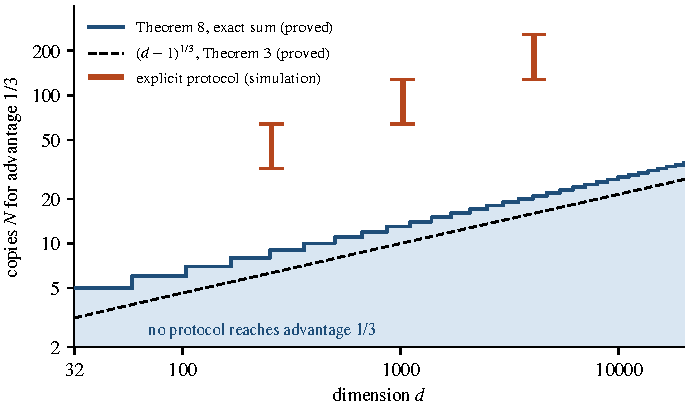
\includegraphics[width=0.64\linewidth]{copies_vs_dimension.pdf}
\caption{Copies needed to reach advantage $1/3$ on the pair of Section~\ref{sec:pair}, which any estimator with error
$\varepsilon<1/8$ and success probability $2/3$ must reach (Lemma~\ref{lem:red}). Below the solid steps (exact sum of Theorem~\ref{thm:bias}) no
single-copy or PPT-BOTH protocol reaches it; the dashed line is the bound $N>(d-1)^{1/3}$ of Theorem~\ref{thm:main}. Bars
span $N=2\sqrt d$ to $4\sqrt d$: the explicit protocol at the end of this section has measured advantage below $1/3$
at the lower end and above it at the upper end (simulation, not used in any proof).}
\label{fig:gap}
\end{figure}

\paragraph{Why summing step norms stops at \texorpdfstring{$d^{1/3}$}{d\textasciicircum(1/3)}} One might hope that computing
the full step norms exactly, instead of bounding them, would improve the exponent. It would not, as long as the steps
are summed with reference $\sigma$: by Proposition~\ref{prop:limit}, for $2\le N\le D$ the coherent steps alone add up to
a quantity between constant multiples of $N^{3/2}/\sqrt D$, and the remaining terms are nonnegative.

\begin{proposition}\label{prop:limit}
For $2\le m\le D$,
\[
\|(X^c_m)^{\Gamma_m}\|_1\ge\|W_m\|_1\ge\frac{\sqrt{m-1}}{2\sqrt{2D}} .
\]
Consequently, for $2\le N\le D$,
\[
\frac{(N-1)^{3/2}}{6\sqrt{2D}}\le\frac12\sum_{m=2}^N\|(X^c_m)^{\Gamma_m}\|_1\le\frac{2N^{3/2}}{3\sqrt{2D}} .
\]
\end{proposition}
\begin{proof}
Let $R:=I^{\otimes(m-1)}\otimes(P-\Pi)$. It is a real diagonal unitary, so conjugation by $R$ commutes with $\Gamma_m$.
In the notation of the splitting, $RA_mR=A_m$, since the last factor of $A_m$ lies in the $\Pi$-block, and
$RB_mR=-B_m$. Therefore $B_m^{\Gamma_m}=(X^c_m)^{\Gamma_m}-R(X^c_m)^{\Gamma_m}R$, which has trace norm at most
$2\|(X^c_m)^{\Gamma_m}\|_1$, and $\|B_m^{\Gamma_m}\|_1=2\|W_m\|_1$ by Lemma~\ref{lem:coh}. For the second inequality,
$L\le m-1\le D$ gives $D+L\le2D$, and $\sqrt x\ge x/\sqrt{m-1}$ on $[0,m-1]$ gives $\E\sqrt{m-1-L}\ge\sqrt{m-1}/2$. The
lower bound on the sum follows from $\sum_{j=1}^{N-1}\sqrt j\ge\frac23(N-1)^{3/2}$. For the upper bound,
Lemmas~\ref{lem:purity} and~\ref{lem:coh} give $\|(X^c_m)^{\Gamma_m}\|_1\le E_m+\|W_m\|_1\le2\sqrt{(m-1)/(2D)}$ when
$m\le D$.
\end{proof}

In particular, for $d\ge6$ and $2(d-1)^{1/3}+1\le N\le d-1$ the coherent step-norm sum alone is at least $1/3$, so this
route cannot certify more than $2(d-1)^{1/3}+2$ copies. This limitation applies only to arguments that bound the
advantage by the sum of the individual partially transposed step norms (Lemma~\ref{lem:tele}) with reference $\sigma$.
It says nothing about other reference states, other groupings of copies, cancellations between different steps, or a
global PPT certificate. Whether the largest PPT-BOTH advantage for this pair is $O(N/\sqrt d+N^2/d)$, which would give
$\Omega(\sqrt d)$, is open.

\paragraph{A failed route} A natural approach through the chain rule would bound how well one more copy can be
distinguished, given the history so far, by the norm of the coherent posterior mean $\E[u\mid\text{history}]$.
Appendix~\ref{app:posterior} shows that this bound is false as stated: the two hypotheses can differ in their posterior
second moments even when the posterior mean is zero.

\paragraph{A numerical check} The simulation described here is not used in any proof. Since the upper bound
of~\cite{du} already implies that this pair can be distinguished with $O(\sqrt d)$ copies, the pair cannot give a lower
bound stronger than $\Omega(\sqrt d)$. To see how an explicit strategy behaves, we simulated one adaptive protocol at
$d\in\{256,1024,4096\}$, with 4000 trials per hypothesis (standard errors $0.008$--$0.011$). The protocol measures half
of the copies in the basis $\{\ket{f_j}\}$ of Section~\ref{sec:two} and sets $w$ to the normalized sum of the observed
vectors $\Pi\ket{f_j}$; if that sum vanishes, $w$ is a fixed unit vector of $\Pi\C^d$ (this never happened in the
runs). It measures the other half in a basis containing $(\ket0\pm\ket w)/\sqrt2$ and decides by the majority sign,
breaking ties with a fair coin (bars in Figure~\ref{fig:gap}). At $N=\sqrt d$, $2\sqrt d$ and $4\sqrt d$ (so
$N/\sqrt{d-1}\approx1$, $2$, $4$) the advantages are about $0.12$--$0.13$, $0.24$--$0.26$ and $0.41$--$0.42$. At each
of these three values the three dimensions agree within $1.4$ combined standard errors (the largest discrepancy over
the whole grid is $2.3$, at $N=\sqrt d/4$). At larger $N$ the advantage levels off near $1/2$, the most this sign test
can reach. These numbers are consistent with the open bound $C(N/\sqrt d+N^2/d)$, but since they only bound the optimal
advantage from below, they are not evidence for it.

\backmatter

\bmhead{Acknowledgements}
The author thanks Ziwei Gu (Harvard John A.\ Paulson School of Engineering and Applied Sciences, Harvard University) for
mentorship and feedback that helped shape this project, for guidance on the research process, and for carefully
verifying the mathematics.

\section*{Statements and Declarations}

\begin{itemize}
\item \textbf{Funding.} No external funding was received for this work; the author funded the project personally.
\item \textbf{Competing interests.} The author declares no competing interests.
\item \textbf{Ethics approval and consent to participate.} Not applicable.
\item \textbf{Consent for publication.} Not applicable.
\item \textbf{Data availability.} The simulation data shown in Figure~\ref{fig:gap} and described in
Section~\ref{sec:discussion}, and the saved outputs of the exact and numerical checks, are openly available at
\url{https://github.com/alex-messerlian/rank-one-overlap-bound}.
\item \textbf{Materials availability.} Not applicable.
\item \textbf{Code availability.} The scripts used for the exact and numerical checks are openly available at
\url{https://github.com/alex-messerlian/rank-one-overlap-bound} under the MIT License.
\item \textbf{Author contributions.} The author initiated and directed the project, proposed the problem from the open
problems of~\cite{du}, revised the text, found errors that were corrected, oversaw all agentic workflows, and
personally funded the project. The author takes full responsibility for the work.
\item \textbf{Use of AI tools.} A single AI model, Anthropic's Claude Opus 5.5, used through the Claude Code
command-line interface for the whole project, derived the results and proofs, wrote the verification code, and drafted
the text.
\end{itemize}

\begin{appendices}

\section{A counterexample to a posterior-coherence route}\label{app:posterior}

Let $d=4$. Measure copies 1 and 2 in the basis $\{\ket{x_\pm}=(\ket0\pm\ket1)/\sqrt2,\ket2,\ket3\}$ and condition on
the history $(x_+,x_-)$. Its probability is $P_c(x_+,x_-)=7/96$ under the coherent ensemble and $P_m(x_+,x_-)=11/96$
under the mixed one. Under $\rho_c(u)$ we have $\langle x_\pm|v\rangle=(1\pm u_1)/2$, where $u_1$ is the coefficient of
$\ket1$, so the likelihood $|\langle x_+|v\rangle|^2|\langle x_-|v\rangle|^2$ is invariant under $u\mapsto-u$ and the
coherent posterior mean $\E[u\mid x_+,x_-]$ vanishes. Nevertheless, the conditional states of copy 3,
\[
\bar\rho_c=\mathrm{diag}\bigl(\tfrac12,\tfrac{13}{70},\tfrac{11}{70},\tfrac{11}{70}\bigr),\qquad
\bar\rho_m=\mathrm{diag}\bigl(\tfrac12,\tfrac{23}{110},\tfrac8{55},\tfrac8{55}\bigr),
\]
differ: the measurement $\{\ket1\bra1,I-\ket1\bra1\}$ gives the distributions $p_c=(\tfrac{13}{70},\tfrac{57}{70})$ and
$p_m=(\tfrac{23}{110},\tfrac{87}{110})$, with $\chi^2(p_c\Vert p_m)=108/32683>0$. Hence no bound of the form
$\chi^2\le C\|\E[u\mid\text{history}]\|^2$ holds. All values are exact rational Haar averages. A similar separation, where one statistic
of the transcript vanishes while another quantity that controls the error terms stays large, appears in certification
lower bounds~\cite[App.~D]{chll}. We include the example only because it rules out this particular route.

\end{appendices}

{\sloppy\begin{thebibliography}{99}\itemsep2pt
\bibitem{du} Z.~Du, Y.~Tang, A.~Elben, I.~Roth, J.~Eisert, Z.~Liu, Optimal randomized measurements for a family of
nonlinear quantum properties, PRX Quantum \textbf{7}, 010360 (2026), \url{https://doi.org/10.1103/4rkx-xkwy};
arXiv:2505.09206v2.
\bibitem{hkp20} H.-Y.~Huang, R.~Kueng, J.~Preskill, Predicting many properties of a quantum system from very few
measurements, Nat.\ Phys.\ \textbf{16}, 1050--1057 (2020), \url{https://doi.org/10.1038/s41567-020-0932-7};
arXiv:2002.08953v2.
\bibitem{hbc22} H.-Y.~Huang, M.~Broughton, J.~Cotler, S.~Chen, J.~Li, M.~Mohseni, H.~Neven, R.~Babbush, R.~Kueng,
J.~Preskill, J.~R.~McClean, Quantum advantage in learning from experiments, Science \textbf{376}, 1182--1186 (2022),
\url{https://doi.org/10.1126/science.abn7293}; arXiv:2112.00778v1.
\bibitem{ye} Q.~Ye, Z.~Liu, D.-L.~Deng, Exponential advantage from one more replica in estimating nonlinear
properties of quantum states, arXiv:2509.24000v1 (2025).
\bibitem{ab} O.~Akresh, J.~Beckey, Tight bounds for purity and product testing from partial transposition,
arXiv:2608.27217v1 (2026).
\bibitem{cchl} S.~Chen, J.~Cotler, H.-Y.~Huang, J.~Li, Exponential separations between learning with and without
quantum memory, in Proc.\ 62nd IEEE Symp.\ Found.\ Comput.\ Sci.\ (FOCS 2021), pp.~574--585,
\url{https://doi.org/10.1109/FOCS52979.2021.00063}; arXiv:2111.05881v2.
\bibitem{lgdc} Z.~Liu, W.~Gong, Z.~Du, Z.~Cai, Exponential separations between quantum learning with and without
purification, arXiv:2410.17718v2 (2024).
\bibitem{ghyz} W.~Gong, J.~Haferkamp, Q.~Ye, Z.~Zhang, Sample complexity of purity and inner product estimation,
Phys.\ Rev.\ Res., accepted (2026), \url{https://doi.org/10.1103/kh2j-jkn6}; arXiv:2410.12712v1.
\bibitem{chll} S.~Chen, B.~Huang, J.~Li, A.~Liu, Tight bounds for quantum state certification with incoherent
measurements, in Proc.\ 63rd IEEE Symp.\ Found.\ Comput.\ Sci.\ (FOCS 2022), pp.~1205--1213,
\url{https://doi.org/10.1109/FOCS54457.2022.00118}; arXiv:2204.07155v2.
\bibitem{clo} S.~Chen, J.~Li, R.~O'Donnell, Toward instance-optimal state certification with incoherent
measurements, in Proc.\ 35th Conf.\ Learning Theory (COLT 2022), PMLR \textbf{178}, pp.~2541--2596;
arXiv:2102.13098v2.
\bibitem{harrow23} A.~W.~Harrow, Approximate orthogonality of permutation operators, with application to quantum
information, Lett.\ Math.\ Phys.\ \textbf{114}, 1 (2024), \url{https://doi.org/10.1007/s11005-023-01744-1};
arXiv:2309.00715v1.
\bibitem{li26} Z.~Li, D.~Chen, D.~Qin, Y.~Yang, Y.~Zhou, Quantum nonlinear properties from a single measurement
setting, arXiv:2605.09958v1 (2026).
\bibitem{afrs} Q.~Liu, Z.~Li, X.~Yuan, H.~Zhu, Y.~Zhou, Auxiliary-free replica shadows: efficient estimation of
multiple nonlinear quantum properties, Phys.\ Rev.\ Lett.\ \textbf{136}, 100602 (2026),
\url{https://doi.org/10.1103/5khs-7dyz}; arXiv:2407.20865v2.
\bibitem{cwyz} K.~Chen, Q.~Wang, Z.~Yu, Z.~Zhang, Simultaneous estimation of nonlinear functionals of a quantum
state, IEEE Trans.\ Inf.\ Theory \textbf{72}(9), 6740--6751 (2026), \url{https://doi.org/10.1109/TIT.2026.3699531};
arXiv:2505.16715v2.
\bibitem{harrow13} A.~W.~Harrow, The church of the symmetric subspace, arXiv:1308.6595v1 (2013).
\end{thebibliography}}
\end{document}
